\section{Block-based Symmetry Breaking}
\label{sec::blocks2}

The idea we develop in this section 
is to store the map in such a way 
that the information can be accessed quickly.  
In particular we want to store together bits of information 
that will be used together, 
so that this information will be retrieve quickly.  
We also show that, in many cases, 
we can avoid looking at nodes individually 
and manipulate groups of nodes in one go.  

\begin{figure}[ht]
  \begin{center}
    \scalebox{0.8}{%
      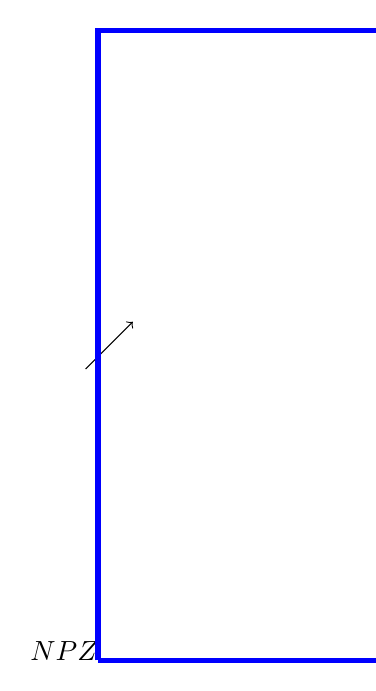
\begin{tikzpicture}
        \creategrid{8}{9}
        \drawobstacle{1}{9}
        \drawobstacle{7}{4}
        \drawobstacle{6}{4}
        \draw[->] (0.7,3.7) -- (1.3,4.3);
        \drawgridnode{2}{5}{$N$}
        \drawgridnode{1}{4}{$P$}
        \drawgridnode{7}{5}{$Z$}
        \drawgridnode{2}{6}{{\color{red} 1}}
        \drawgridnode{1}{5}{{\color{red} 2}}
        \drawgridnode{3}{5}{{\color{red} 3}}
        \drawgridnode{2}{7}{{\color{red} 4}}
        \drawgridnode{1}{6}{{\color{red} 5}}
        \drawgridnode{3}{6}{{\color{red} 6}}
        \drawgridnode{2}{8}{{\color{red} 7}}
        \drawgridnode{1}{7}{{\color{red} 8}}
        \drawgridnode{3}{7}{{\color{red} 9}}
        \draw[blue,line width=2pt] (0,0) -- (0,8) -- (4,8) -- (4,0) -- (0,0);
      \end{tikzpicture}%
    }
  \end{center}
  \caption{A current search state 
    (the grid is assumed larger than the part presented).
  The red numbers show in which order the traversability of the nodes 
  is tested.}
  \label{fig::gridforblocks}
\end{figure}

Consider the grid presented on Figure~\ref{fig::gridforblocks} 
(this is supposed to be a small chunk of a larger grid).  
The node currently being explored in $N$ ($\langle 2,5\rangle$)
and its parent is $P$.  
At this stage, the horizontal and vertical axes must be scanned 
for jump point before a diagonal move to $\langle 3,6\rangle$ is taken.  
As it turns out, a jump point will be found in $Z$.  
When looking for a jump point on column $2$, 
the status (traversable or not) of the nodes 
will be checked in the order given by the numbers in red.  
This information is most likely scattered in the memory 
which means many memory cache misses and less efficient access.  

We therefore propose to put all these nodes in the same 32-bit word.  
For instance, all the nodes in the blue rectangle, 
i.e., defined by the corners $\langle 1,1\rangle$ 
and $\langle 4,8\rangle$.  
Even more, because there is no obstacle in the 32-bit word, 
a single check (\emph{does the word equal to 0?}) 
allows to immediately jump to node $\langle 2,9\rangle$.  

An obvious issue with this approach 
is that, while the blue rectangle allows 
to quickly search on columns $2$ and $3$, 
it is not convenient for, say, columns $1$ and $4$ or any row.  
Consequently, we propose to add redundancy in the map as follows: 
\begin{itemize}
\item 
  We build ``horizontal'' rectangles 
  to quickly search over rows, 
  for instance a rectangle between corners 
  $\langle 0,0\rangle$ and $\langle 8,4\rangle$.  
  This doubles the size of the map.    
\item 
  We build overlaping rectangles 
  for those columns and rows that border the rectangles, 
  for instance a rectangle between corners 
  $\langle 2,0\rangle$ and $\langle 6,8\rangle$.  
  This doubles again the size of the map.  
\end{itemize}

%EOF 
